%% LaTeX Beamer presentation template (requires beamer package)
%% see http://bitbucket.org/rivanvx/beamer/wiki/Home
%% idea contributed by H. Turgut Uyar
%% template based on a template by Till Tantau
%% this template is still evolving - it might differ in future releases!

\documentclass{beamer}

\mode<presentation>
{
\usetheme{Warsaw}

\setbeamercovered{transparent}
}

\usepackage{../../Common/sty/TI84} %TODO: How to get the link working...?



\title{Masterclass programmeren op de GR TI-84 (les 2)}

%\subtitle{}

% - Use the \inst{?} command only if the authors have different
%   affiliation.
%\author{F.~Author\inst{1} \and S.~Another\inst{2}}
\author{Kevin van As}

% - Use the \inst command only if there are several affiliations.
% - Keep it simple, no one is interested in your street address.
% \institute[Universities of]
% {
% \inst{1}%
% Department of Computer Science\\
% Univ of S
% \and
% \inst{2}%
% Department of Theoretical Philosophy\\
% Univ of E}

\date{\today}


% This is only inserted into the PDF information catalog. Can be left
% out.
\subject{Masterclass GR TI-84 programmeren (les 2)}



% If you have a file called "university-logo-filename.xxx", where xxx
% is a graphic format that can be processed by latex or pdflatex,
% resp., then you can add a logo as follows:

% \pgfdeclareimage[height=0.5cm]{university-logo}{university-logo-filename}
% \logo{\pgfuseimage{university-logo}}



% Delete this, if you do not want the table of contents to pop up at
% the beginning of each subsection:
\AtBeginSubsection[]
{
\begin{frame}<beamer>
\frametitle{Outline}
\tableofcontents[currentsection,currentsubsection]
\end{frame}
}

% If you wish to uncover everything in a step-wise fashion, uncomment
% the following command:

%\beamerdefaultoverlayspecification{<+->}

\begin{document}

\begin{frame}
\titlepage
\end{frame}


\begin{frame}
\frametitle{Recap!}

\visible<2>{\ticalcfig{\ticalcfigCircle{\ticalcfigCircleColThree}{0.615}}} % prgm
\visible<3-4>{\ticalcfig{\ticalcfigCircle{\ticalcfigCircleColFour}{0.62}}} % Vars
\visible<5>{\ticalcfig{\ticalcfigCircle{\ticalcfigCircleColThree}{0.615}}} % prgm

We hebben gekeken naar:
\begin{itemize}
	\item<2-> Waar kun je prgms vinden?
	\item<3-> Wat zijn variabelen?
	\item<4-> \lenitem{Wat zijn datatypen? \\ Met namen: getallen en strings.}
	\item<5-> \lenitem{Basic I/O: \tifonttxt{Prompt} en \tifonttxt{Disp}.}
\end{itemize}
\end{frame}

\begin{frame}
\frametitle{Vooruitzicht!}

Vandaag zullen we kijken naar:
\begin{itemize}
	\item<2-> Boolean datatype
	\item<3-> Control: ``\tifonttxt{If} statements''
	\item<4-> Pseudo Code
	\item<5-> Algoritmes
\end{itemize}

\end{frame}


%% END %%

\begin{frame}
\frametitle{Outline}
\tableofcontents
% You might wish to add the option [pausesections]
\end{frame}

% The core pages
\section{Datatype: Boolean}


\begin{frame}
\frametitle{Wat is een Boolean?}

\begin{itemize}
  \item<1-> Een Boolean datatype beschrijft een waarheid,
  			of of er aan een conditie voldaan wordt: ``Juist'' of ``Onjuist''
  \begin{itemize}
    \item<2-> In het Engels, ``True'' of ``False''
  \end{itemize}
  \item<3-> Een Boolean kan dus slechts twee waarden aannemen: \\ Hij is ``Binair'',
  			en is dus ook te beschouwen als een Binair getal: 1 (juist) of 0 (onjuist).
  \item<4-> De Boolean wordt ook gebruikt in de Logica om op een formele manier
  			te redeneren over de juistheid van argumenten.		
\end{itemize}

\end{frame}





\begin{frame}
\frametitle{Wat is het nut van een Boolean?}

Booleans kunnen gebruikt worden om je programma te conditioneren:

Onder bepaalde voorwaarden (condities) heeft je programma een andere output.

\vspace{0.5cm}
\pause %1
Neem bijvoorbeeld de ABC formule:

\pause %2
Afhankelijk van
\only<5->{\underline{het teken van de discriminant}}\only<1-4>{het teken van de discriminant}
zijn er nul, een of twee oplossingen.

$D=b^2-4ac$

\vspace{0.3cm}
\pause %3
Wat is hier de conditie?
\pause %4

\end{frame}





\begin{frame}
\frametitle{Voorbeelden van statements}

Condities zijn statements zoals:

\inlineticalc{C=2} \inlineticalc{\pi\!3} \inlineticalc{A>6} \inlineticalc{A<B} \inlineticalc{X\ge42} \inlineticalc{0\le A}

\uncover<2->{Vraag: Wanneer zijn deze 6 condities ``true''?}

\visible<3->{
\begin{itemize}
  \item \tifonttxt{=} Gelijk aan.
  \item \tifonttxt{\!} Ongelijk aan.
  \item \tifonttxt{>} Groter dan.
  \item \tifonttxt{<} Kleiner dan.
  \item \tifonttxt{\ge} Groter dan of gelijk aan.
  \item \tifonttxt{\le} Kleiner dan of gelijk aan.
\end{itemize}
}

\end{frame}












% EOF
\section{If-statements}


\begin{frame}
\frametitle{Hoe kunnen we condities gebruiken in een programma?}

Allereerst\ldots Hoe gebruiken we condities in ons taalgebruik?

\vspace{15pt}
\visible<2->{``Als het regent, dan blijf ik binnen.''}

\visible<3->{``Als ik later groot ben, dan wordt ik een brandweerman.''}

\visible<4->{``Als ik die toets haal, dan ga ik over, of anders blijf ik zitten.''}

\vspace{15pt}
\visible<5->{In het algemeen:\\
``\textbf{Als} <<CONDITIE>>, \textbf{dan} <<ACTIE>>, \textbf{of anders} <<ACTIE>>''}

\end{frame}




\begin{frame}
\frametitle{Hoe kunnen we condities gebruiken in een programma?}

\visible<1->{``\textbf{Als} <<CONDITIE>>, \textbf{dan} <<ACTIE>>, \textbf{of anders} <<ACTIE>>. \textbf{Klaar}.''}

\vspace{3pt}
\visible<2->{``\textbf{If} <<CONDITION>>, \textbf{then} <<ACTION>>, \textbf{else} <<ACTION>>. \textbf{End}.''}

\vspace{15pt}
\visible<3->{
\begin{minipage}{0.43\textwidth}%
	\only<-4>{
		\begin{ticalc}[4.3cm]
			PROGRAM\:FIRST IF\\%
			\:If\,SOME\,CONDITION\\%
			\:Then\\%
			\:DO\,SOMETHING\\%
			\:Else\\%
			\:DO\,OTHER\,THING\\%
			\:End
		\end{ticalc}
	}\only<5->{
% 		\begin{figure}
% 			\hspace{-1.2cm}
% 		  	\centering
% 		    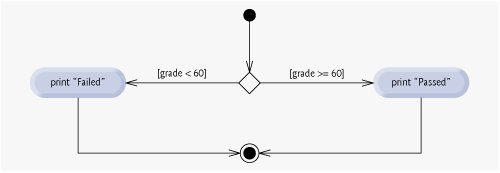
\includegraphics[width=1.2\textwidth]{../figures/IfDiagram.jpg}
% 		\end{figure}
		\begin{tikzpicture}[overlay,remember picture]
			\node [anchor=west,xshift=-0.9cm,yshift=0cm]
			{
			\begin{tikzonimage}[width=1.2\textwidth]{../figures/IfDiagram.jpg}
			\end{tikzonimage}
			};
		\end{tikzpicture}
	}
\end{minipage}%
~
\visible<4->{
\begin{minipage}{0.53\textwidth}%
	\begin{ticalc}[5.3cm]
		PROGRAM\:FIRST IF\\%
		\:If\,G\ge60\\%
		\:Then\\%
		\:Disp\,\qt PASSED.\qt\\%
		\:Else\\%
		\:Disp\,\qt FAILED.\qt\\%
		\:End
	\end{ticalc}
\end{minipage}%	
}
}

\vspace{5pt}
\visible<5->{Er ontstaan nu twee paden in het programma:\\}
\visible<6->{Slechts de statement(s) tussen \tifonttxt{Then} en \tifonttxt{Else} wordt uitgevoerd,
of de statement(s) tussen \tifonttxt{Else} en \tifonttxt{End}.}
\visible<7->{Daarna gaat het programma verder met statements die onder \tifonttxt{End} staan.}



% \begin{tikzpicture}[overlay,remember picture]
% 	\node[] (SE) at (current page.south east){ };
% 	\node [anchor=south east,xshift=0.05cm,yshift=1.4cm] at (SE)
% 	{
% 	\begin{tikzonimage}[height=#1]{../figures/IfDiagram.jpg}
% 	\end{tikzonimage}
% 	};
% \end{tikzpicture}

\end{frame}






\begin{frame}
\frametitle{Waar staat het op de GR?}

\visible<1-2,6->{\ticalcfig{\ticalcfigCircle{\ticalcfigCircleColThree}{0.615}}} % prgm
\visible<3>{\ticalcfig{}} % nothing
\visible<4-5>{\ticalcfig{\ticalcfigCircleSecond\ticalcfigCircle{\ticalcfigCircleColOne}{0.64}}} % test menu

\begin{itemize}
  \item<1-> Maak een nieuw programma: \inlineticalc{PROGRAM\:FIRSTIF}.
  \item<2-> Druk op \tiPRGM\,en kies \tifonttxt{If}.
  \item<3-> Type een letter.
  \item<4-> Druk op \tiTEST=\tiSecond\tiMATH\,en kies \tifonttxt{=}.
  \item<5-> Type \tifonttxt{0} gevolgd door \tiENTER.
  \item<6-> Druk op \tiPRGM\,en kies \tifonttxt{Then}, daarna \tiENTER.
  \item<7-> Druk op \tiPRGM\,en kies \tifonttxt{Else}, daarna \tiENTER.
  \item<8-> Druk op \tiPRGM\,en kies \tifonttxt{End}, daarna \tiENTER.
  \item<9-> Dit is de structuur van het \tifonttxt{if}-statement.
\end{itemize}


\begin{tikzpicture}[overlay,remember picture]
	\node[] (BL) at (current page.south east){ };
	\node [anchor=south east,xshift=0.195cm,yshift=0.6cm] at (BL)
	{%
	\only<1,3,5,9>{%
		\begin{ticalc}
			PROGRAM\:FIRSTIF\\%
			\:\only<1>{\tiCursor}\visible<3->{If\,A\only<3>{\tiCursor}\visible<5->{=0\\%
			\:\only<5>{\tiCursor}}}\visible<9->{Then\\%
			\:Else\\%
			\:End}\\%
			\visible<0>{.}
		\end{ticalc}
	}%
	\only<2>{%
		\begin{ticalc}
			\select{CTL}\,I/O\,EXEC \\
			\selectitem{1\+\:}If \\
			2\:Then \\
			3\:Else \\
			4\:For( \\
			5\:While \\
			6\:Repeat( \\
			7\arrowdown End
		\end{ticalc}
	}%
	\only<4>{%
		\begin{ticalc}
			\select{TEST}\,LOGIC \\
			\selectitem{1\+\:}= \\
			2\:\! \\
			3\:> \\
			4\:\ge \\
			5\:< \\
			6\:\le
		\end{ticalc}
	}%
	\only<6>{%
		\begin{ticalc}
			\select{CTL}\,I/O\,EXEC \\
			1\+\:If \\
			\selectitem{2\:}Then \\
			3\:Else \\
			4\:For( \\
			5\:While \\
			6\:Repeat( \\
			7\arrowdown End
		\end{ticalc}
	}%
	\only<7>{%
		\begin{ticalc}
			\select{CTL}\,I/O\,EXEC \\
			1\+\:If \\
			2\:Then \\
			\selectitem{3\:}Else \\
			4\:For( \\
			5\:While \\
			6\:Repeat( \\
			7\arrowdown End
		\end{ticalc}
	}%
	\only<8>{%
		\begin{ticalc}
			\select{CTL}\,I/O\,EXEC \\
			1\+\:If \\
			2\:Then \\
			3\:Else \\
			4\:For( \\
			5\:While \\
			6\:Repeat( \\
			\selectitem{7\arrowdown} End
		\end{ticalc}
	}%
	};
\end{tikzpicture}

\end{frame}





\begin{frame}
\frametitle{Intermezzo: Invoegen/Insert}

\visible<3,5->{\ticalcfig{\ticalcfigCircleSecond\ticalcfigCircle{\ticalcfigCircleColThree}{0.8}}} % Ins
\visible<4>{\ticalcfig{\ticalcfigCircleSecond\ticalcfigCircle{\ticalcfigCircleColThree}{0.8}\ticalcfigCircleEnter}} % Ins + Enter
\visible<1,2>{\ticalcfig{}} % nothing

\begin{itemize}
  \item<2-> \lenitem{Plaats je cursor op \tifonttxt{Else}.}
  \item<3-> \lenitem{Druk op \tiINS=\tiSecond\tiDEL. Je cursor is nu verandert.}
  \item<4-> \lenitem{Druk op \tiENTER. Je hebt nu een regel \textit{boven} ingevoegd.}
  \item<5-> \lenitem{\tiINS=\tiSecond\tiDEL\,of de cursor bewegen be\"eindigd de insert-modus.}
\end{itemize}

\begin{tikzpicture}[overlay,remember picture]
	\node[] (BL) at (current page.south east){ };
	\node [anchor=south east,xshift=0.195cm,yshift=0.6cm] at (BL)
	{%
	\only<1>{%
		\begin{ticalc}
			PROGRAM\:FIRSTIF\\%
			\:If\,A=0\\%
			\:Then\\%
			\:Else\\%
			\:End\\%
			\visible<0>{.}
		\end{ticalc}
	}%
	\only<2>{%
		\begin{ticalc}
			PROGRAM\:FIRSTIF\\%
			\:If\,A=0\\%
			\:Then\\%
			\:\tiCursor lse\\%
			\:End\\%
			\visible<0>{.}
		\end{ticalc}
	}%
	\only<3>{%
		\begin{ticalc}
			PROGRAM\:FIRSTIF\\%
			\:If\,A=0\\%
			\:Then\\%
			\:\_lse\\%
			\:End\\%
			\visible<0>{.}
		\end{ticalc}
	}%
	\only<4>{%
		\begin{ticalc}
			PROGRAM\:FIRSTIF\\%
			\:If\,A=0\\%
			\:Then\\%
			\:\\%
			\:\_lse\\%
			\:End
		\end{ticalc}
	}%
	\only<5->{%
		\begin{ticalc}
			PROGRAM\:FIRSTIF\\%
			\:If\,A=0\\%
			\:Then\\%
			\:\\%
			\:Else\\%
			\:End
		\end{ticalc}
	}%
	};
\end{tikzpicture}


\end{frame}



\begin{frame}
\frametitle{Oefening!}

TODO: OEFENINGEN IN DE KLAS
%TODO

\end{frame}








\section{Pseudocode \& Algoritmes}
\subsection{Uitleg}

\begin{frame}
\frametitle{Hoe zet je een probleem om in een programma?}

\begin{itemize}
  \item<1-> Begin met het probleem te versimpelen.
  \item<2-> Denk vervolgens als een computer:
  \begin{itemize}
  	\item<3-> Niets is ``duidelijk'' of ``obvious'': 
	  \begin{itemize}
	  	\item<4-> De computer denkt niet zelf na!
	  \end{itemize}
  	\item<5-> Je moet alles letterlijk uitspellen voor de computer!
  \end{itemize}
  \item<6-> Het helpt om gebruik te maken van ``pseudocode''.
\end{itemize}

\end{frame}



\begin{frame}
\frametitle{Wat is pseudocode?}

\begin{itemize}
  \item<1-> Pseudocode ligt tussen ``echte'' code en mensentaal in.
  \begin{itemize}
  	\item<2-> ``Echte'' code heeft een strakke syntax waar je je aan moet houden.
  	\begin{itemize}
  	  \item<3-> Een kleine typefout en de computer begrijpt je niet!
  	\end{itemize}
  	\item<4-> Pseudocode heeft niet zo'n strakke syntax,\\maar het is ``in eigen woorden''
  \end{itemize}
  \item<5-> Pseudocode heeft echter wel de \textbf{structuur} van een stukje code
\end{itemize}

\end{frame}




\begin{frame}
\frametitle{Wat is pseudocode?}
\framesubtitle{Voorbeeld}

Stel dat we een programma willen schrijven die ons vertelt of we vandaag een paraplu nodig hebben.
\visible<2>{In pseudocode:}


\visible<2->{
\begin{minipage}{0.7\textwidth}%
	\begin{algorithm}[H]
	\caption{Pseudocode ``paraplu nodig?''}
	\begin{algorithmic}[1]
	\Function{ParapluNodig}{regenkans}
	   \If{regenkans = hoog}
	     \State Paraplu nodig
	   \ElsIf{regenkans = laag}
	     \State Geen paraplu nodig
	   \Else
	     \State Paraplu optioneel. \Comment{Je smelt niet!}
	   \EndIf
	\EndFunction
	\end{algorithmic}
	\end{algorithm}
\end{minipage}%
\visible<3->{
\begin{minipage}{0.27\textwidth}%
	\begin{ticalc}
		PROGRAM\:PARAPLU\\%
		\:Prompt\,R\\%
		\:If\,R>40\\%
		\:Then\\%
		\:Disp\,\qt PARAPLU\,NODIG\qt\\%
		\:Else\:If\,R<10\\%
		\:Then\\%
		\:Disp\,\qt PARAPLU\,ONNODIG\qt\\%
		\:Else\\%
		\:Disp\,\qt PARAPLU\,OPTIONEEL\qt\\%
		\:End
		\:End
	\end{ticalc}
\end{minipage}%	
}
}


\addtocounter{algorithm}{-1} % Prevents the algorithm number to increase every frame
\end{frame}
\addtocounter{algorithm}{1} % Make sure the number increases for a new algorithm on a different slide


\begin{frame}
\frametitle{Wat is het nut van pseudocode?}

Wanneer een programma zeer ingewikkeld wordt, kun je soms honderden regels code samenvatten in slechts 1 zin pseudocode.
Bijv. ``bereken het elektrisch veld'', zoals in de figuur hieronder.

\visible<2->{
\begin{figure}[h]
\centering
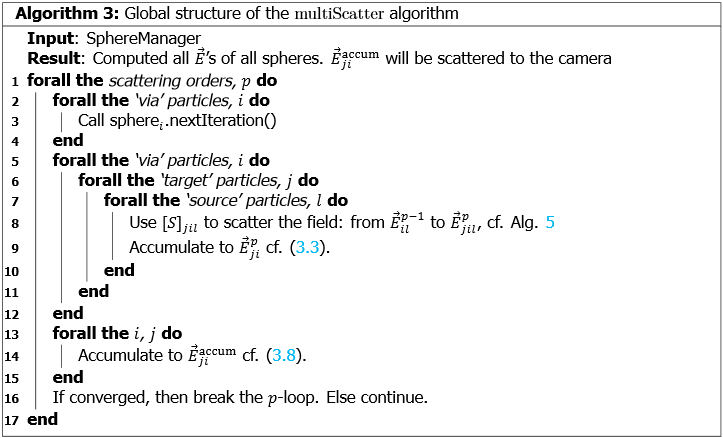
\includegraphics[height=0.6\textheight]{../figures/AlgorithmMScThesis.png}
\end{figure}
\tiny{Deze figuur komt uit mijn master afstudeerproject: http://www.kevinvanas.nl/TUDelft/MSc/Report.pdf}
}

\end{frame}


\begin{frame}
\frametitle{Wat is een algoritme?}

\begin{itemize}
  \item<1-> Op voorgaande slides kwam het woord ``\textbf{Algorithm}'' voor (NL: Algoritme). Wat is dat?
  \item<2-> Een algorithme is ``een stukje code''.
  \item<3-> Dat ``stukje code'' heeft als doel om iets specifieks uit te rekenen.
  \begin{itemize}
    \item<4-> Bijvoorbeeld het uitrekenen van het zesde priemgetal\only<5->{ ($=13$)}.
  \end{itemize}
  \item<5-> Dus overal waar ``Algorithm'' staat, kun je simpelweg denken ``\emph{een stukje computercode om iets uit te rekenen}''.
\end{itemize}

\end{frame}


\subsection{Zelf Oefenen}

\begin{frame}
\frametitle{Oefening: Wat doet deze pseudocode?}

\begin{algorithm}[H]
\caption{Pseudocode ``WhatDoIDo?''}
\begin{algorithmic}[1]
% ABC formule
\Function{WhatDoIDo}{$a$,$b$,$c$}
	\State $D=\sqrt{b^2-4ac}$
	\If{$D>0$}
		\State Er zijn twee oplossingen
		\State $x = (-b\pm D) / 2a$
	\ElsIf{$D=0$}
		\State Er is exact \'e\'en oplossing
		\State $x = -b / 2a$
	\Else \Comment{$D<0$}
		\State Er zijn geen re\"ele oplossingen!
	\EndIf
\EndFunction
\end{algorithmic}
\end{algorithm}

\end{frame}




\begin{frame}
\frametitle{Oefening: Wat doet deze pseudocode?}

\begin{algorithm}[H]
\caption{Pseudocode ``WhatDoIDo2?''}
\begin{algorithmic}[1]
% Risk dobbelstenen
\Function{WhatDoIDo2}{$N_{att}$}
	\State Maak $N_{att}$ random getallen tussen $1$ en $6$
	\State Vraag of $N_{def}$ $1$ of $2$ is
	\State Maak $N_{def}$ random getallen tussen $1$ en $6$
	\State Sorteer beide setten van hoog naar laag
	\If{Getal 1 van set 1 > Getal 1 van set 2}  $p_1=p_1+1$
	\Else \hspace{0.4cm} $p_2=p_2+1$
	\EndIf
	\If{Getal 2 van set 1 > Getal 2 van set 2}  $p_1=p_1+1$
	\Else \hspace{0.4cm} $p_2=p_2+1$
	\EndIf
	\State Display de scores: $p_1$ en $p_2$
\EndFunction
\end{algorithmic}
\end{algorithm}


\end{frame}




\begin{frame}
\frametitle{Oefening: Wat doet deze pseudocode?}

\begin{algorithm}[H]
\caption{Pseudocode ``WhatDoIDo3?''}
\begin{algorithmic}[1]
% Spraakherkenning
\Function{WhatDoIDo3}{geluid $g$}\Comment{Niet voor GR geschikt}
\State Knip $g$ op in losse klanken, $k$.
\State Laad een database in.
\State Verwijder de stiltes uit $k$.
\State Correleer $k$ met alle items in de database.
\State Bereken een score voor alle klanken en vind daarmee de meest waarschijnlijke letter.
\State Maak een lijst voor alle mogelijke woorden die $g$ kan zijn.
\State Vergelijk de lijst met een woordenboek en kies het meest waarschijnlijke woord.
\EndFunction
\end{algorithmic}
\end{algorithm}


\end{frame}



\begin{frame}\label{frame:pseudo_exercises}
\frametitle{Nu jullie: Maak je eigen pseudocode!}

\begin{enumerate} 
  \item Bepaal of iemand genoeg geld, $g$, op zijn rekening heeft staan, indien hij een product voor $x$ euro wil kopen
  	en $r$ euro in het rood mag staan.
  \item Gegeven de huidige datum, $(y_t, m_t, d_t)$, en iemand's geboortedatum, $(y_g, m_g, d_g)$, bepaal zijn/haar leeftijd.
  \item Uit een set van 5 kaarten, bepaal wat de pokerset is.
  \begin{itemize}
    \item Bijvoorbeeld: ``pair of $5$'s, $K$ high'' or ``straight, $9$ high''
  \end{itemize}
  \item Er zijn vier spelers die elk punten hebben. Bepaal de winnaar, i.e. degene met de meeste punten.
  \item Bereken de `rest' van $y/x$.
  \begin{itemize}
    \item Bijvoorbeeld: $5/2 = 2$ `rest' $1$
    \item Tip: Kijk naar \tiMATH\inlineticalc{NUM}\inlineticalc{int(} of \tiMATH\inlineticalc{NUM}\inlineticalc{fPart(}
  \end{itemize}
\end{enumerate}

\end{frame}






\begin{frame}
\frametitle{Zet pseudocode om in een \tifonttxt{Prgm}!}

Implementeer deze twee opdrachten van de vorige slide op je rekenmachine:

\begin{enumerate} 
  \item Bepaal of iemand genoeg geld, $g$, op zijn rekening heeft staan, indien hij een product voor $x$ euro wil kopen
  	en $r$ euro in het rood mag staan.
  \item Gegeven de huidige datum, $(y_t, m_t, d_t)$, en iemand's geboortedatum, $(y_g, m_g, d_g)$, bepaal zijn/haar leeftijd.
  \begin{itemize}
    \item Tip: Het is handig om voor jezelf duidelijk 6 variabelen te kiezen \emph{\'en} op te schrijven wat alles betekent.
    	Immers, je kunt slechts \'e\'en letter gebruiken per variabele! Duidelijkheid is zeer belangrijk:
    	Als je het overzicht verliest, dan weet je zeker dat je je \tifonttxt{Prgm} niet kunt schrijven.
  \end{itemize}
\end{enumerate}



\end{frame}






\section{Exercises}

\begin{frame}
\frametitle{Exercises}

Maak de pseudocodes en implementeer alle algoritmes van slide \ref{frame:pseudo_exercises}
(dat zijn de opdrachten aan het einde van ``pseudocode \& algoritmes''), voor in hoeverre je kunt.

De pokeropdracht is optioneel. Ik raad aan om w\'el de pseudocode te maken, maar het niet te implementeren.
Dat is gigantisch veel werk op je GR.
% Tip voor de pokeropdracht: Gebruik twee variabelen per kaart (dus 10 in totaal).
% \'E\'en voor het nummer (1 tot 13), en \'e\'en voor de kleur (harten, ruiten, schoppen, klaveren).

\end{frame}

%
% \begin{enumerate} 
%   \item Bepaal of iemand genoeg geld, $g$, op zijn rekening heeft staan, indien hij een product voor $x$ euro wil kopen
%   	en $r$ euro in het rood mag staan.
%   \item Gegeven de huidige datum, $(y_t, m_t, d_t)$, en iemand's geboortedatum, $(y_g, m_g, d_g)$, bepaal zijn/haar leeftijd.
%   \item Uit een set van 5 kaarten, bepaal wat de pokerset is.
%   \begin{itemize}
%     \item Bijvoorbeeld: ``pair of $5$'s, $K$ high'' or ``straight, $9$ high''
%   \end{itemize}
%   \item Er zijn vier spelers die elk punten hebben. Bepaal de winnaar, i.e. degene met de meeste punten.
%   \item Bereken de `rest' van $y/x$.
%   \begin{itemize}
%     \item Bijvoorbeeld: $5/2 = 2$ `rest' $1$
%     \item Tip: Kijk naar \tiMATH\inlineticalc{NUM}\inlineticalc{int(} of \tiMATH\inlineticalc{NUM}\inlineticalc{fPart(}
%   \end{itemize}
% \end{enumerate}
%


\begin{frame}
\frametitle{Antwoorden}

\begin{minipage}{0.4\textwidth}
\begin{ticalc}
	PROGRAM\:NUFMONEY\\%
	\:Input\,\qt HOEVEEL\,GELD?\,\qt\comma G\\%
	\:Input\,\qt HOEVEEL\,KOST\,HET?\,\qt\comma X\\%
	\:Input\,\qt HOEVEEL\,KREDIET?\,\qt\comma R\\%
	\:\\%
	\:If\,G-X\ge0\:Then\\%
	\:Disp\,\qt JE\,KUNT\,HET\,BETALEN\qt\\%
	\:Else\\%
	\:If\,X-G>R\:Then\\%
	\:Disp\,\qt TE\,DUUR\qt\\%
	\:Else\\%
	\:Disp\,\qt OK,\,KOST\,KREDIET\qt\\%
	\:End
\end{ticalc}
\end{minipage}
\begin{minipage}{0.4\textwidth}
\begin{ticalc}[5cm]
	PROGRAM\:BIRTHDAY\\%
	\:Input\,\qt YOU\,Y\qt\comma Y\\%
	\:Input\,\qt YOU\,M\qt\comma M\\%
	\:Input\,\qt YOU\,D\qt\comma D\\%
	\:Input\,\qt CUR\,Y\qt\comma Z\\%
	\:Input\,\qt CUR\,M\qt\comma N\\%
	\:Input\,\qt CUR\,D\qt\comma E\\%
	\:\\%
	\:Z-Y\>A\\%
	\:If\,M>N\:Then\\%
	\:A+1\>A\\%
	\:Else\\%
	\:If\,M=N\,and\,D>E\:Then\\%
	\:A-1\>A\\%
	\:End\\%
	\:End\\%
	\:Disp\,A
\end{ticalc}
\end{minipage}

\end{frame}



\begin{frame}
\frametitle{Antwoorden}

\begin{minipage}{0.48\textwidth}
Dit negeert gelijkspel\ldots En is slecht leesbaar.
Later meer over dit soort gevallen (m.b.v. Lists).

\vspace{0.2cm}
\begin{ticalc}
	PROGRAM\:WIEWINT\\%
	\:Prompt\,A\\%
	\:Prompt\,B\\%
	\:Prompt\,C\\%
	\:Prompt\,D\\%
	\:\\%
	\:If\,A>B\:Then\\%
		\:If\,A>C\:Then\\% A or D win
			\:If\,A>D\:Then\\%
				\:Disp\,\qt A\,WINS\qt\\%
			\:Else\\%
				\:Disp\,\qt D\,WINS\qt\\%
			\:End\\%
		\:Else\\% C or D win
			\:If\,C>D\:Then\\%
				\:Disp\,\qt C\,WINS\qt\\%
\end{ticalc}
\end{minipage}
~
\begin{minipage}{0.48\textwidth}
\begin{ticalc}	
			\:Else\\%
				\:Disp\,\qt D\,WINS\qt\\%
			\:End\\%		
		\:End\\%
	\:Else\\% A does not win
		\:If\,B>C\:Then\\% B or D win
			\:If\,B>D\:Then\\%
				\:Disp\,\qt B\,WINS\qt\\%
			\:Else\\%
				\:Disp\,\qt D\,WINS\qt\\%
			\:End\\%
		\:Else\\% C or D win
			\:If\,C>D\:Then\\%
				\:Disp\,\qt C\,WINS\qt\\%
			\:Else\\%
				\:Disp\,\qt D\,WINS\qt\\%
			\:End\\%
		\:End\\%
	\:End
\end{ticalc}
\end{minipage}

\end{frame}




% \begin{frame}
% \frametitle{Antwoorden}
% 
% \begin{minipage}{0.4\textwidth}
% \begin{ticalc}
% 	PROGRAM\:POKER\\%
% 	\,Input\,\qt NUM1\qt\comma A\\%
% 	\,Input\,\qt COL1\qt\comma B\\%
% 	\,Input\,\qt NUM2\qt\comma C\\%
% 	\,Input\,\qt COL2\qt\comma D\\%
% 	\,Input\,\qt NUM3\qt\comma E\\%
% 	\,Input\,\qt COL3\qt\comma F\\%
% 	\,Input\,\qt NUM4\qt\comma G\\%
% 	\,Input\,\qt COL4\qt\comma H\\%
% 	\,Input\,\qt NUM5\qt\comma I\\%
% 	\,Input\,\qt COL5\qt\comma J\\%
% \end{ticalc}
% \end{minipage}
% \begin{minipage}{0.4\textwidth}
% \begin{ticalc}
% \end{ticalc}
% \end{minipage}
% 
% \end{frame}



\begin{frame}
\frametitle{Antwoorden}

\begin{ticalc}[5cm]
	PROGRAM\:RESTYDX\\%
	\:Disp\,\qt REST(Y/X)\:\qt\\%
	\:Input\,\qt Y=\qt\comma Y\\%
	\:Input\,\qt X=\qt\comma X\\%
	\:If\,X=0\\%
	\:Then\\%
	\:Disp\,\qt X\,CANNOT\,BE\,0\qt\\%
	\:Stop\\%
	\:End\\%
	\:Disp\,fPart(Y/X)*X\\%
	\:Disp\,(Y/X-int(Y/X))*X%
\end{ticalc}

\end{frame}










\end{document}

%% END %%